\documentclass[9pt, a4paper, notitlepage]{extreport}
\usepackage[T1]{fontenc}
\usepackage[utf8]{inputenc}
\usepackage{amssymb,amsmath}
\usepackage[brazil]{babel}
\usepackage{comment}
\usepackage{datetime}
\usepackage[colorlinks=true]{hyperref}
\usepackage{graphicx}
\usepackage{multicol}
\usepackage{fancyhdr}
\usepackage[table]{xcolor}
\usepackage{enumitem}

% --- Configuração de Margens compactas ---
\usepackage[a4paper, landscape, left=0.5cm, right=0.5cm, top=1.2cm, bottom=0.8cm]{geometry}

% --- Configuração do MINTED (compacto) ---
\usepackage{minted}
\usemintedstyle{bw}  % Estilo preto e branco, mais compacto

% Opções globais para minted - máxima compactação
\setminted{
    fontsize=\small,
    tabsize=2,
    breaklines,
    breakanywhere,
    autogobble,
    frame=none,
    framesep=0pt,
    xleftmargin=0pt,
    numbersep=2pt,
    baselinestretch=0.8
}

% Remove espaçamento extra
\setlength{\parindent}{0pt}
\setlength{\parskip}{0pt}
\setlength{\columnsep}{8pt}
\setlength{\columnseprule}{0.2pt}

% Configuração de cabeçalho e rodapé
\pagestyle{fancy}
\fancyhf{}
\fancyhead[L]{\small UFRJ -- Meu nome é shadow. Sou aquele que deixou todo o seu passado para trás. Não faço esse contest por ninguém, não estou preso a nada}
\fancyhead[R]{\small\thepage}
\renewcommand{\headrulewidth}{0.4pt}
\setlength{\headheight}{12pt}

% Compactar seções
\usepackage{titlesec}
\titlespacing*{\section}{0pt}{4pt plus 2pt minus 2pt}{2pt plus 1pt minus 1pt}
\titlespacing*{\subsection}{0pt}{3pt plus 1pt minus 1pt}{1pt plus 1pt minus 1pt}
\titleformat{\section}{\normalfont\large\bfseries}{\thesection}{1em}{}
\titleformat{\subsection}{\normalfont\normalsize\bfseries}{\thesubsection}{0.8em}{}

% Compactar TOC
\usepackage{tocloft}
\setlength{\cftbeforesecskip}{1pt}
\setlength{\cftbeforesubsecskip}{0pt}
\renewcommand{\cftsecfont}{\small}
\renewcommand{\cftsubsecfont}{\footnotesize}
\renewcommand{\cftsecpagefont}{\small}
\renewcommand{\cftsubsecpagefont}{\footnotesize}

\begin{document}

% Include cover page
\begin{titlepage}
    \pagestyle{empty}
	\begin{center}
		\strut % Magic
		
		\includegraphics[width=9cm]{Imagens/projeto.png}
		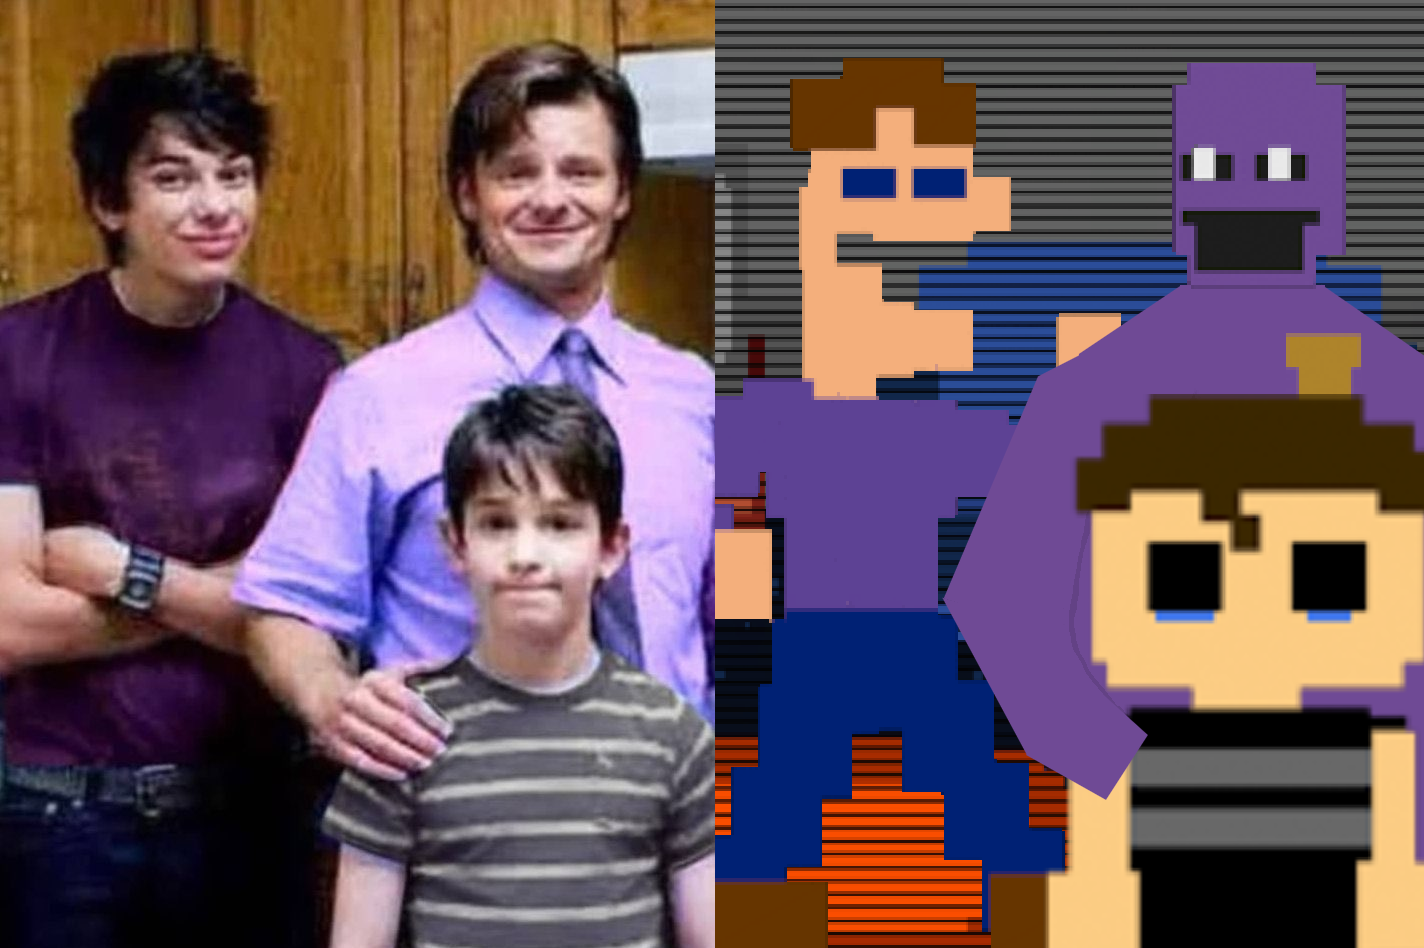
\includegraphics[width=10cm]{Imagens/DWKFNAF.png}\\[1cm]
		{\fontsize{25}{30}\selectfont Universidade Federal do Rio de Janeiro\\[0.8cm]}
		{\fontsize{40}{30}\selectfont \textbf{www.paraosdebaixo.com.br}\\[0.8cm]}
		{\fontsize{20}{20}\selectfont{Enzo Vieira, Caio David, Luís Rafael}\\}
		% \vfill
		\vspace{2.5cm}
		{\fontsize{20}{20}\selectfont{Agosto, 2026}}\\
		\vspace{1cm}
    \end{center}
\end{titlepage}

\begin{multicols}{2}
% \tableofcontents
\end{multicols}

\vspace{2mm}

\begin{multicols}{3}
